\chapter{Tientsin} 

\subsection{TS Type 4}
\begin{figure}[htbp]
\centering
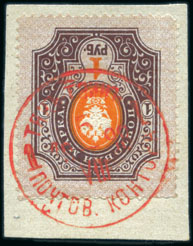
\includegraphics[width=.50\textwidth]{../russian-post-offices-in-china/10008.jpg}
\caption{
10008	TIENTSIN: 1899 1R tied on piece by Tientsin 8.12.97 type 4 cds in red, 
very fine
\euro 80.00
}  
\end{figure}

\begin{figure}[htbp]
\centering
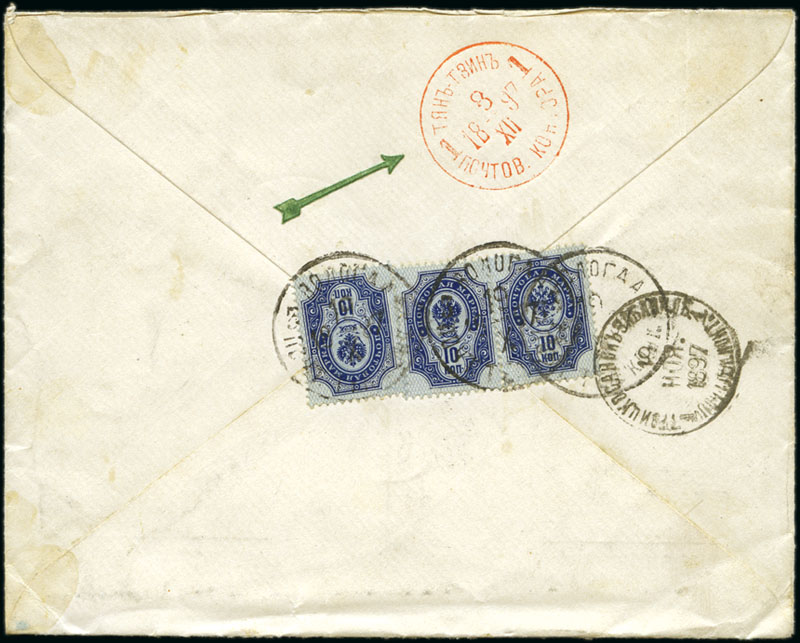
\includegraphics[width=.95\textwidth]{../russian-post-offices-in-china/10007.jpg}
\caption{
10007 TIENTSIN INCOMING: 1897 Cover from Vologda to the Russian Consul-General
in Shanghai, franked on the reverse with three 10k, with Troitskosavsk 
and Russian Tientsin 8.12.97 type 4 cds in red adjacent
\euro 200.00 
}  
\end{figure}

\begin{figure}[htbp]
\centering
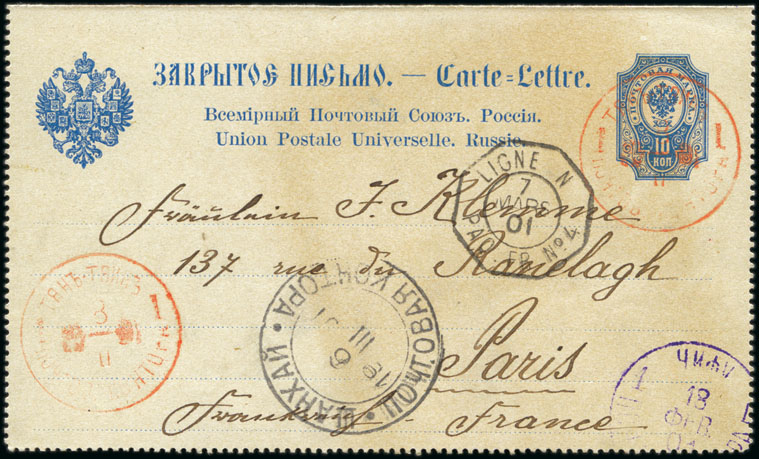
\includegraphics[width=.95\textwidth]{../russian-post-offices-in-china/10009.jpg}
\caption{
10009		ZoomTIENTSIN: 1901 Ordinary Russian 10k letter-card to France
cancelled by Tientsin 8.2.1901 cds in red (T\&S type 4X, characterised
by defective year numerals), with Chefoo Russian P.O. transit in violet 
(Tchil. type 2), Shanghai Russian P.O. cds (Gregorian calendar) and French 
paquebot ds, a rare usage of postal stationery
\euro 400.00 
}  
\end{figure}

\begin{figure}[htbp]
\centering
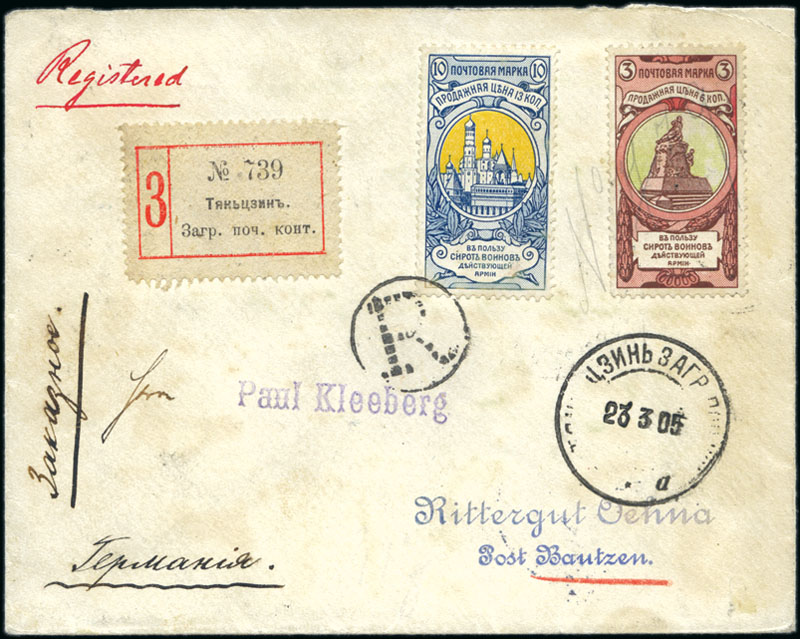
\includegraphics[width=.95\textwidth]{../russian-post-offices-in-china/10010.jpg}
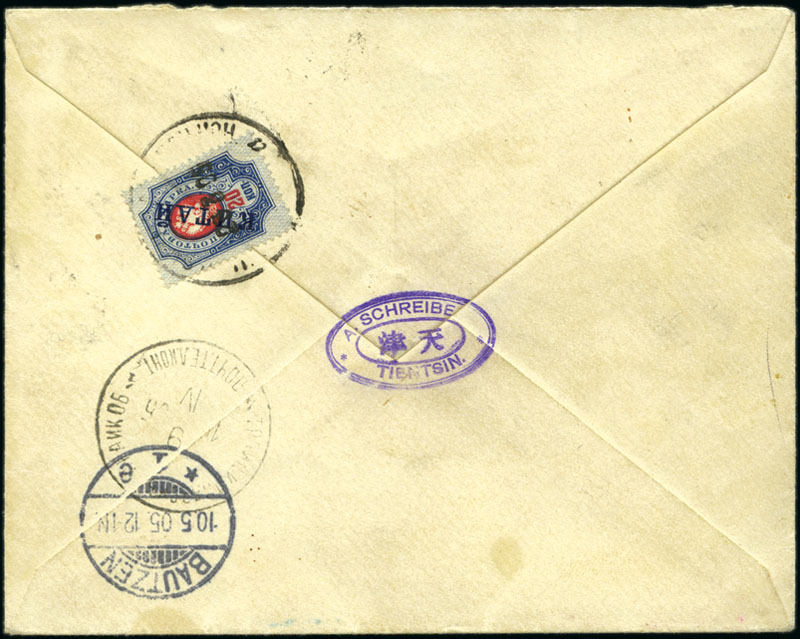
\includegraphics[width=.95\textwidth]{../russian-post-offices-in-china/10010-1.jpg}
\caption{
10010	TIENTSIN: 1905 Cover sent registered to Germany franked on the reverse
with "KITAI" 20k tied by Tientsin 23.3.05 cds (Tchilinghirian type 5A), 
and franked on the obverse with War Charity 10k and 3k that were 
ignored by the P.O. as a philatelic embellishment, with the 10k tied only 
by the encircled "dotted R" hs, registered label adjacent, Troitskosavsk 
transit indicating that it was not sent by the Trans-Siberian railway 
via Manchuria (as it was closed during the Russo-Japanese War), very unusual.
Note: The War Charity issue was not distributed to the P.O.s in China.
\euro 600.00
}  
\end{figure}






                                